% !TeX root = main.tex

\chapter{Back Propagation Through Time}
L'algorithme BPTT appliqué à un réseau neuronal récurrent a pour particularité
de déplier le temps dans l'espace; par exemple, pour apprendre un mot de cinq
caractères, on va créer cinq réseaux non-récurrents qui représentent chaqun un
"temps", soit une lettre de la séquence. \\

Cet algorithme a pour avantage, par rapport à celui RTRL, d'avoir une
complexité temporelle inférieure.

\section{Théorie}

\begin{figure}[!ht]
\begin{center}
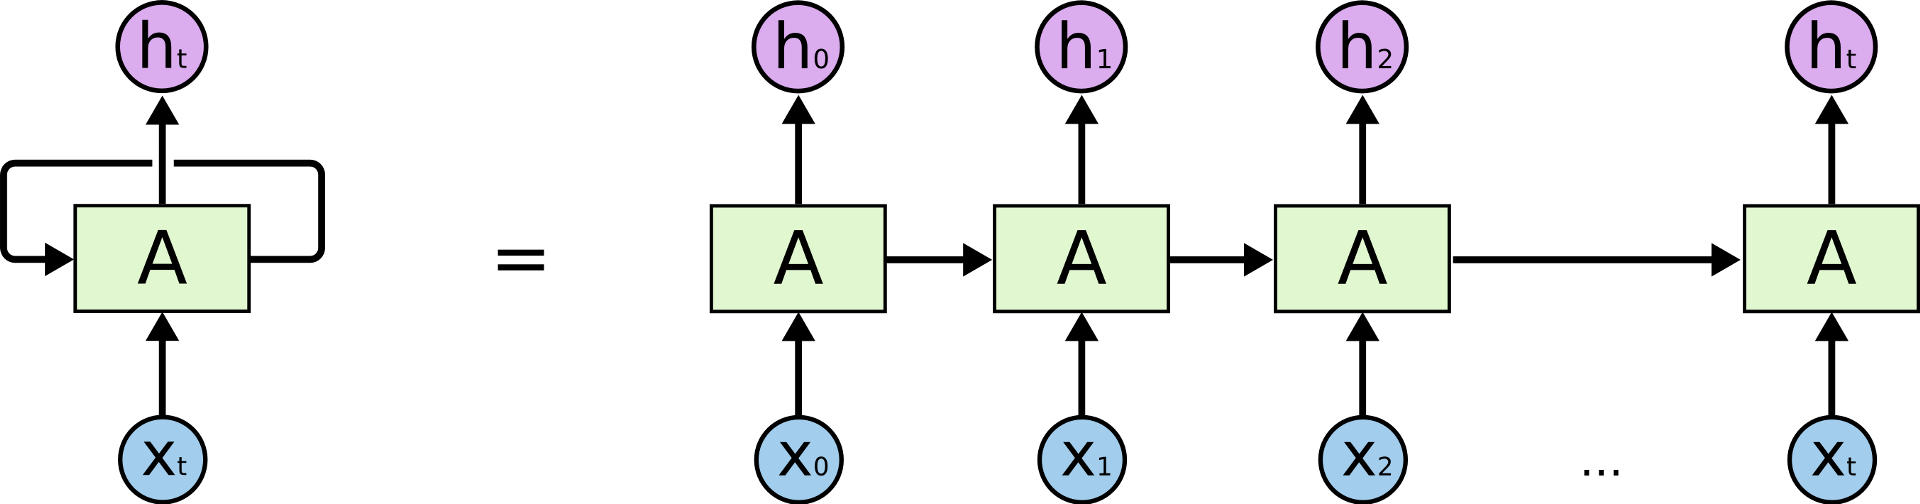
\includegraphics[scale=0.2]{images/bptt.png}
\end{center}
\caption{Dépliement du temps dans l'espace pour BPTT}
\end{figure}

\subsection{Réseau BPTT}

\section{Implémentation}

\section{Résultats}
\subsection{Grammaire de Reber simple}
\subsection{Grammaire de Reber double}
